\begin{savequote}[8cm]
Conoscere nel senso della Scienza vuol dire prevedere.

To know in its Scientific meaning, means to predict.
  \qauthor{--- Carlo Rubbia}
\end{savequote}

\chapter{\label{ch:3-DUNE}The Deep Underground Neutrino Experiment}


\minitoc
\section{Introduction} \label{ch3-Sec:Introduction}
\begin{figure}[!ht]
     \centering
     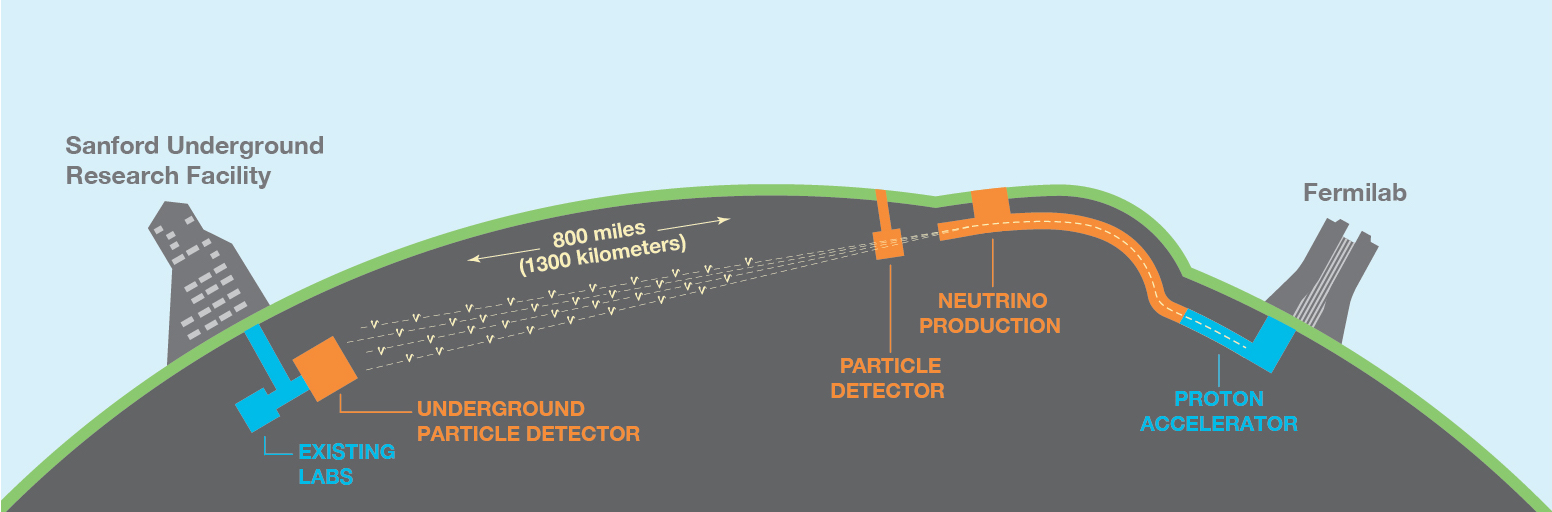
\includegraphics[width=0.99\textwidth]{figures/ch3-DUNE/LBNE_Graphic_061615_2016.jpg}
     \caption{Schematic representation of the DUNE experiment with its main components}
        \label{fig:DUNEdiagram}
\end{figure}
The Deep Underground Neutrino Experiment (DUNE) will be a next generation long baseline neutrino oscillation experiment \cite{DUNE:2020TDR1}. Its main goal will be to measure all the parameters governing neutrino and anti-neutrino oscillations in a single experiment, with particular emphasis on the CP violation phase $\delta_\textrm{CP}$ and the neutrino mass ordering. The experiment will consist of three main components: a wide band high intensity neutrino beam situated at Fermilab, which will be capable of producing both a $\nu_\mu$ and a $\Bar{\nu}_\mu$ fluxes; a kt-scale underground liquid Argon based Far Detector (FD), situated at the Sanford Underground Research Facility (SURF) in South Dakota, at $\sim1300$ Km from the source; a modular Near Detector (ND) situated at $\sim500$ m from the source.

Due to budgetary restrictions DUNE will pursue a staged approach in its construction and data production \cite{DUNE:2022Snowmass}. The initial composition of the experiment, referred to as Phase I, will include two LArTPC Far Detector modules, both being 10kt in volume, but utilizing a Vertical Drift \cite{DUNE:2023TDRVD} and an Horizontal Drift (or Single Phase) technology \cite{DUNE:2020TDR4} respectively. The initial configuration of the ND will include two out of the three originally envisioned detectors: the liquid argon near detector ND-LAr, a modular LArTPC similar in technology to the FD modules and the system for on axis neutrino detection SAND, whose main function will be to act as a beam monitor \cite{Battisti:2022ND}. A third ND module will be placed between ND-LAr and SAND to act as a muon spectrometer: this will be called the Temporary Muon Spectrometer (TMS) and will be removed from the ND facilities after Phase I to be replaced by a more capable detector. In Phase I DUNE will be able to determine the neutrino mass ordering, measure $\delta_\textrm{CP}$ at 3$\sigma$ if maximal, measure several oscillation parameters at world-leading levels of precision, detect supernova collapse neutrinos if available and search for BSM physics. 

In order to pursue its full physics scope, after Phase I DUNE will undertake several key improvements to all of its key components: this second form of the experiment is referred to as Phase II. The Far Detector will be completed by two extra liquid argon modules (nominally using the Verdical Drift technology) for a total fiducial mass of at least 40kt. The proton beam's power will augmented from 1.2 MW to 2.4 MW. The TMS will be replaced by a more capable high pressure gaseous Argon magnetized detector called ND-GAr. All of these upgrades are necessary for DUNE to reach one of its key stated goals: reach 5$\sigma$ sensitivity on CP violation over a wide range of $\delta_\textrm{CP}$ values. Additionally in Phase II, DUNE will be capable of producing independent measurements of $\sin^2{\theta_{13}}$ with precision comparable to that of reactors, it will have significant sensitivity to the $\theta_{23}$ octant, and will reach a world-leading sensitivity in a wide range of physics beyond the three neutrino paradigm as well as additional BSM physics and astrophysics. 

\section{DUNE's facilities and design}
\subsection{The LBNF beamline}
\begin{figure}[!h]
     \centering
     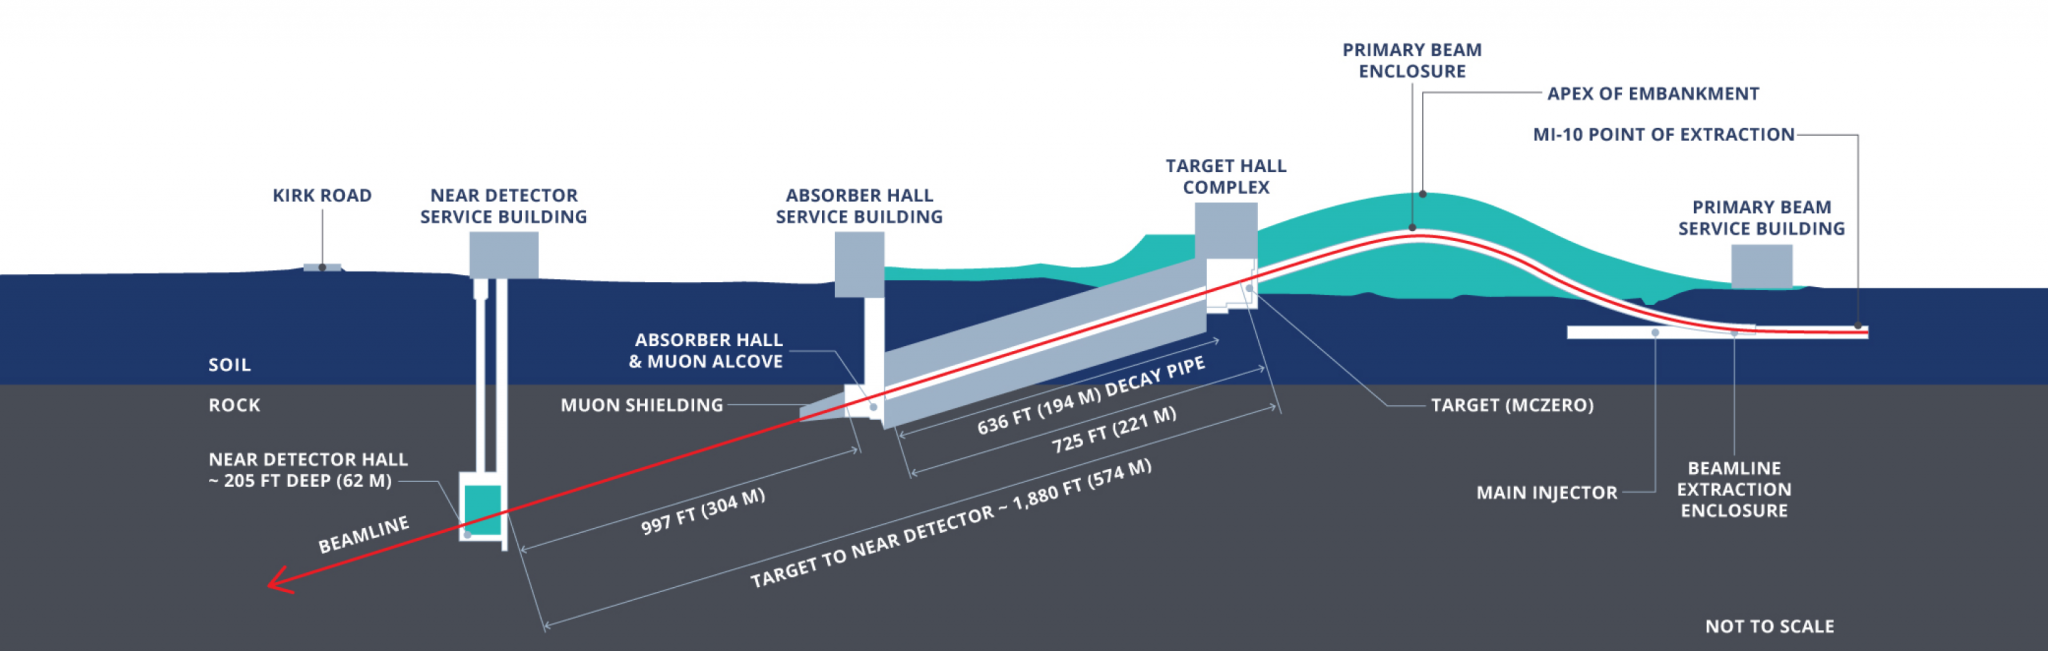
\includegraphics[width=0.99\textwidth]{figures/ch3-DUNE/LBNF-IL-graphic-Fermilab-LBNF.png}
     \caption{Schematic representation of the DUNE experiment with its main components}
        \label{fig:KFdiagram}
\end{figure}
The neutrino flux that will be utilized by the DUNE experiment, will be produced by the LBNF Beamline at Fermilab, which is expected to produce the highest power neutrino beam in the world \cite{DUNE:2016LBNFTDR, Papadimitriou:2016ksv}. The production of the neutrino flux begins by accelerating protons through a proton accelerator. The primary proton beam, which operates in the energy range of 60-120 GeV, is extracted from Fermilab's Main Injector (MI), a proton accelerator already utilized by the NOvA experiment and partially based on the Tevatron collider facilities. The main injector will be upgraded through the Proton Improvement Plan, phase II (PIP-II), in time for the DUNE Phase I data taking period to reach average beam powers of the order of 1.14 MW, delivering $7.5 \times 10^{13}$ protons in one MI machine cycle (0.7 sec - 1.2 sec) to the LBNF target. Further improvements are expected the PIP III project to reach 2.4 MW of power for DUNE Phase II and all the beamline components are being planned to accommodate these improvements with minimal retro-fitting. 

Once the primary proton beam reaches the desired energy, it is directed through the use of extraction and transport components over a man-made hill and bent downwards towards a graphite target located at grade level. This constitutes the first element of the proper neutrino beamline. The charged mesons, primarily kaons and pions, produced in the interactions of the protons are sign selected and focused by two magnetic horns into a decay pipe toward the far detector. The target and focusing horns are all located inside a heavily shielded vault called the target chase, that is isolated from the decay pipe at its downstream end by a metallic window. Their design is derived from that of the NuMi neutrino beam. 

The mesons produced in the proton interactions are short-lived and decay into either anti-muons and neutrinos or muons and anti-neutrino,s depending on the charge of the mesons. If the main neutrino types being produced are $\nu_\mu$ the Beamline is said to be in Forward Horn Current (FHC) mode, otherwise it is said to be in Reverse Horn Current (RHC) mode.  Both polarities will produced high purity
fluxes, with an expected contamination from the “incorrect” neutrino type (i.e. $\nu_\mu$ in RHC mode and vice-versa) of less than 10\% in the oscillation energy region. This type of impurities are introduced by hadrons of the opposite sign propagating at the centre of the beam, where no magnetic field is present. A small $\nu_e$ and $\Bar{\nu}_e$
component is also introduced by the decay of secondary kaons and tertiary muons from pion decays. At the end of the decay region, an absorber is needed to remove the residual hadrons remaining at the end of the decay pipe.  The absorber core consists of replaceable aluminium and steel water-cooled blocks. Approximately 40\% of the beam power is deposited in the target chase and surrounding shielding, 30\% in the decay pipe and 30\% in the absorber.

The wide band neutrino beam which is produced by the Beamline facilities, is needed to cover the first and second neutrino oscillation maxima, which for a 1300 km baseline are expected to be approximately at 2.4 and 0.8 GeV. For this reason the beamline design is optimized for neutrino energies between 0.5 and 5 GeV. 

\subsection{The Far Detector}
\begin{figure}[!ht]
     \centering
     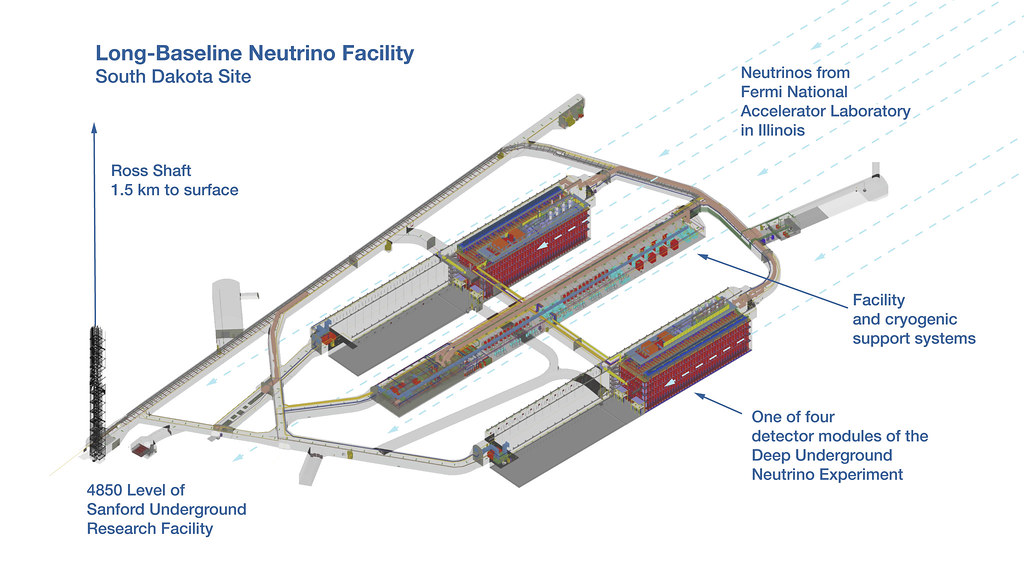
\includegraphics[width=0.99\textwidth]{figures/ch3-DUNE/Far_Detector.jpg}
     \caption{Schematic representation of the Far Detector experiment with its main components}
        \label{fig:DUNEdiagram}
\end{figure}
The DUNE Far Detector will be composed of four LArTPC detector module, each containing a 10kt fiducial liquid Argon mass  and a total liquid Argon mass of 17.5kt. Each module will fit inside a cryostat. Of the four modules only the first two will be available during DUNE Phase I, the first one using an Horizontal Drift technology (originally identified as Single Phase \cite{DUNE:2020TDR4}) will be called FD1-HD and the second one using a Vertical Drift technology\cite{DUNE:2023TDRVD} (evolved from the Dual Phase Technology \cite{DUNE:2018mlo}) will be called FD2-VD. The last two modules will be employed during Phase II and are nominally set to be Vertical Drift detectors\cite{DUNE:2022Snowmass}.

The LArTPC was pioneered by the ICARUS experiment \cite{Rubbia:1977zz,ICARUS:2004wqc} and is now a mature detector technology within the neutrino experiment community, being employed in detectors such as MicroBooNe\cite{MicroBooNE:2016pwy} and SBND\cite{Machado:2019oxb} at Fermilab as well as the ProtoDUNE-SP\cite{DUNE:2020cqd} prototype tested at the CERN neutrino facilities. In a LArTPC, ionization electrons produced by the energy deposition of charged particles generated in neutrino interactions, are drifted by an electric field in the liquid Argon towards an anode and are collected on a charge multiplier element, producing a readable two dimensional signal. The measurement of the collected ionization electrons also provides a measurement of the $dE/dx$ of the charged particles, which is what enables both calorimetry and particle identification (PID) in a LArTPC.

Argon is a UV light scintillator. Once shifted into the visible spectrum, the UV scintillation photons produced by can be collected by photon detectors and provide an initial start time $t_0$, indicating when the ionization electrons begin to drift. Comparing the time at which the ionization signal reaches the anode relative to this start time allows reconstruction of the event topology in the drift coordinate. 

The FD1-HD design combines a kt level fiducial mass with a sub-cm spacial resolution. Both are crucial to achieve DUNE's scientific goals of measuring CP violation, while searching for nucleon decay and being capable of observing neutrinos from supernova bursts. An example of the design of the detector being directly informed by the physics requirements of the experiment, comes from the electron/photon separation requirements necessary to study $\nu_e$ appearance signals in the LBNF $\nu_\mu$ flux. Electrons are typically produced in charged current $\nu_e$ interactions and induce electro-magnetic showers in the LAr medium. Similar electro-magnetic activity can be induced by photons coming for example from $\pi^0$ decay. The FD modules are capable of distinguishing between these two signals by using $dE/dx$ information combined with spacial information. Photon induced signals have an initial non ionized gap of several cm's before the formation of the electro-magnetic shower and have a $dE/dx$ which is double that of an electron induced one.

\begin{figure}[!t]
     \centering
     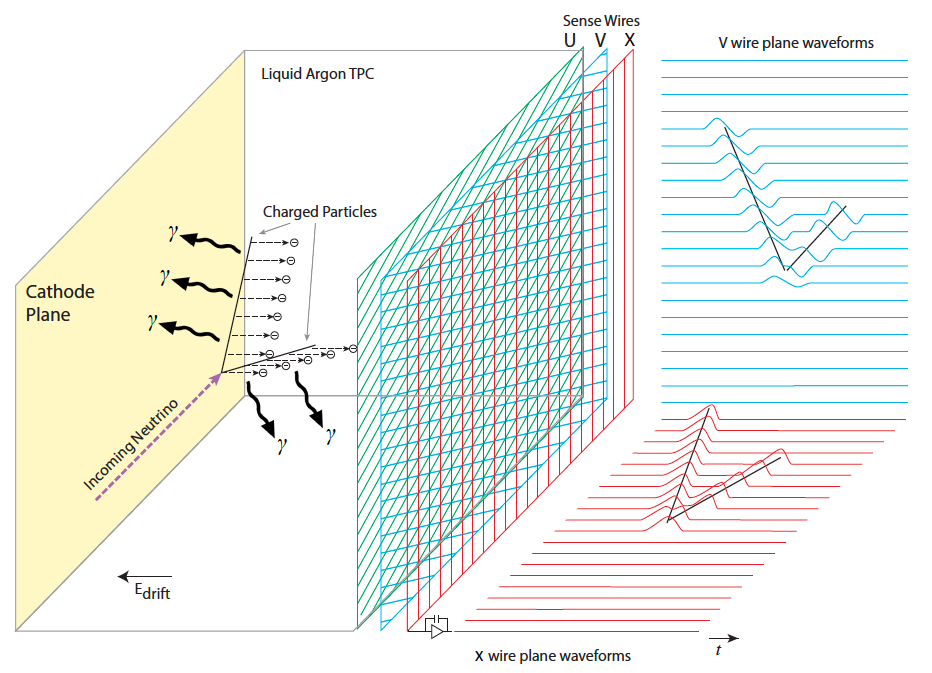
\includegraphics[width=0.8\textwidth]{figures/ch3-DUNE/TheBoPicture.png}
     \caption{Schematic representation of the Far Detector experiment with its main components}
        \label{fig:DUNEdiagram}
\end{figure}

The FD1-HD detector modules consist of 4 separate liquid Argon filled drift volumes with a maximum drift length of 3.5 m. Each Volume is instrumented with a vertical cathode plane and an anode plane, for a total of three module-long (58.2 m) anode planes and two cathode planes. A field cage covers the spaces between the two, producing a stable 500 V/m electric field in the horizontal direction. The drift ionization electrons reach the anode planes in an order of a few milli-seconds. 

Each anode plane is instrumented with a total of 50 anode plane assemblies APAs which consist of an aluminum frame with three layers of active wires and an additional shielding layer wrapped around them. The first two active layers are identified as the U and V induction layers. These layers are angled at a $\pm 37.5^\circ$ in order to reduce ambiguities in event reconstruction. The relative voltage between the layers is chosen so that the drift electrons pass through them and produce a bipolar induction signal on both planes. The drifting electrons are finally collected in the final $X$ wire plane, where they produce a mono-polar signal. In the $X$ collection plane, as well as in the $G$ shielding plane, the wires run vertically. The spacing between the wires in each layer is of 5 mm, and defines the spacial resolution of the APAs.

The scintillation photons produced by the passing charged particles in the liquid Argon in the very ultra violet (VUV) spectrum are collected by photon detector (PD) systems called X-ARAPUCA \cite{Segreto:2018jdx}. The photons are produce in the order of 24000 per MeV of deposited energy, and reach the detectors in a time-frame of the order of a nanosecond. The X-ARAPUCA modules are mounted between the sets of wire-planes and consist of layers of dichroic filter and wavelength shifters, that shift the VUV scintillation light into the visible range, trap the visible photons, and transport them to a silicon photo-multiplier (SiPM). The signals produced in the SiPMs are then combined with the wire signals from the APAs at the data acquisition (DAQ) level.

\begin{figure}[!t]
     \centering
     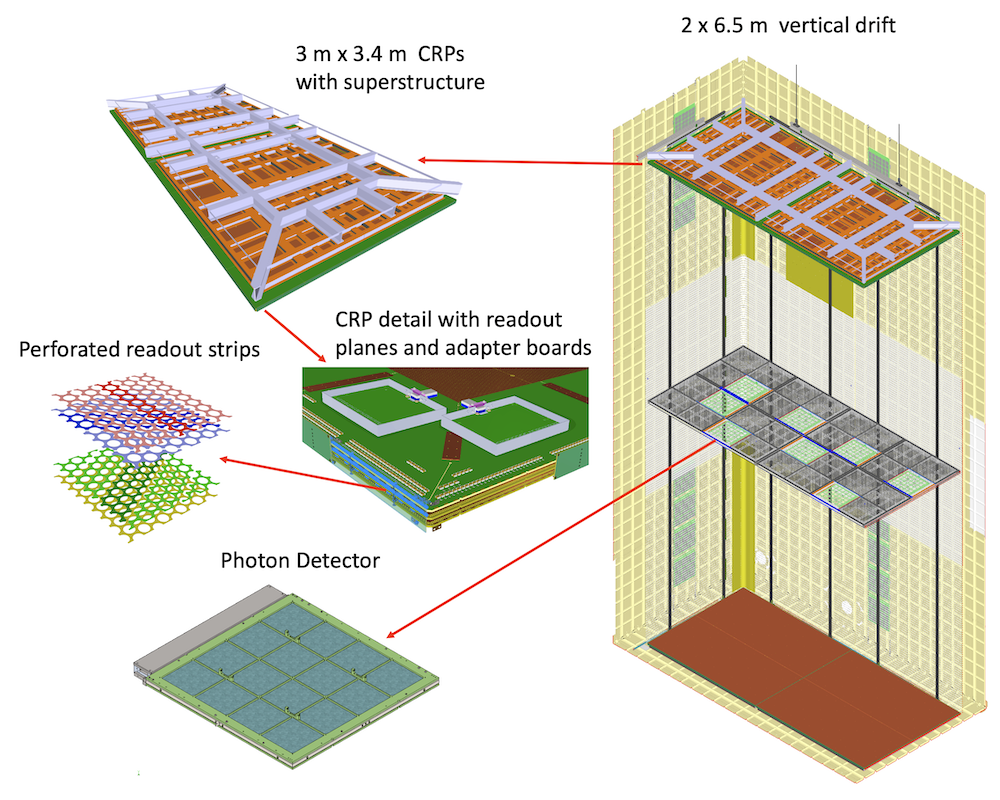
\includegraphics[width=0.7\textwidth]{figures/ch3-DUNE/setup_new_updated.png}
     \caption{Schematic representation of the Far Detector experiment with its main components}
        \label{fig:DUNEdiagram}
\end{figure}

The FD2-VD design has developed from the R\&D experience accumulated by the DUNE collaboration with the ProtoDUNE-SP and ProtoDUNE-DP prototypes at the neutrino research facilities at CERN. The detector consists of several vertical drift modules enclosed in a large cryostat structure. Each module is divided into two vertical drift regions 6.5 m in height, by an horizontal cathode and feature two anode planes, one close to the cryostat top, just below the surface of the liquid Argon region and one close to the bottom of the cryostat. Field cage modules hang vertically around the module's perimeter. The 450 V/cm electric field drifts the ionisation electrons, either upwards or downwards depending on the drift region. The vertical design of the FD2-VD offers a slightly larger instrumented module compared to FD1-HD and it's more cost-effective thanks to its high-modularity and general structure and geometry. 

The anode planes in the FD2-VD design consist of two double-sided perforated printed circuit boards (PCBs) that are connected to form a charge-readout unit (CRUs). The perforation holes allow the electrons to pass through the PCB's. The first PCB is instrumented with two sets of induction strips, while the second one hosts the collection strips. The three planes of strips are segmented at about 7.5 mm pitch for the induction planes and 5 mm pitch for the collection plane, and are set at $60^\circ$ angles relative to each other to maximize information in the charge readout from different projections. Two CRU's are connected to a frame to form a Charge Readout Plane (CRP). Each anode plane consists of 80 CRP's. Much like in the FD1-HD design the anode plane signal allows for a two-dimensional reconstruction of any given event, while the third dimension is given by the drift time information obtained from the scintillation light.

The PD's implemented in the FD2-VD follow the same general design of the ARAPUCA-X modules developed for FD1-HD. The PDs will be mounted on the four cryostat membrane walls as on both sides of the central cathode structure. This configuration offers a uniform ligth measurement coverage across the entire LArTPC volume. Additionally, the FD2-VD liquid argon will be doped with a small quantity of xenon. This has no impact on the TPC operation but significantly enhances the photon detection performance.

\subsection{The Near Detector}

\begin{figure}[!h]
     \centering
     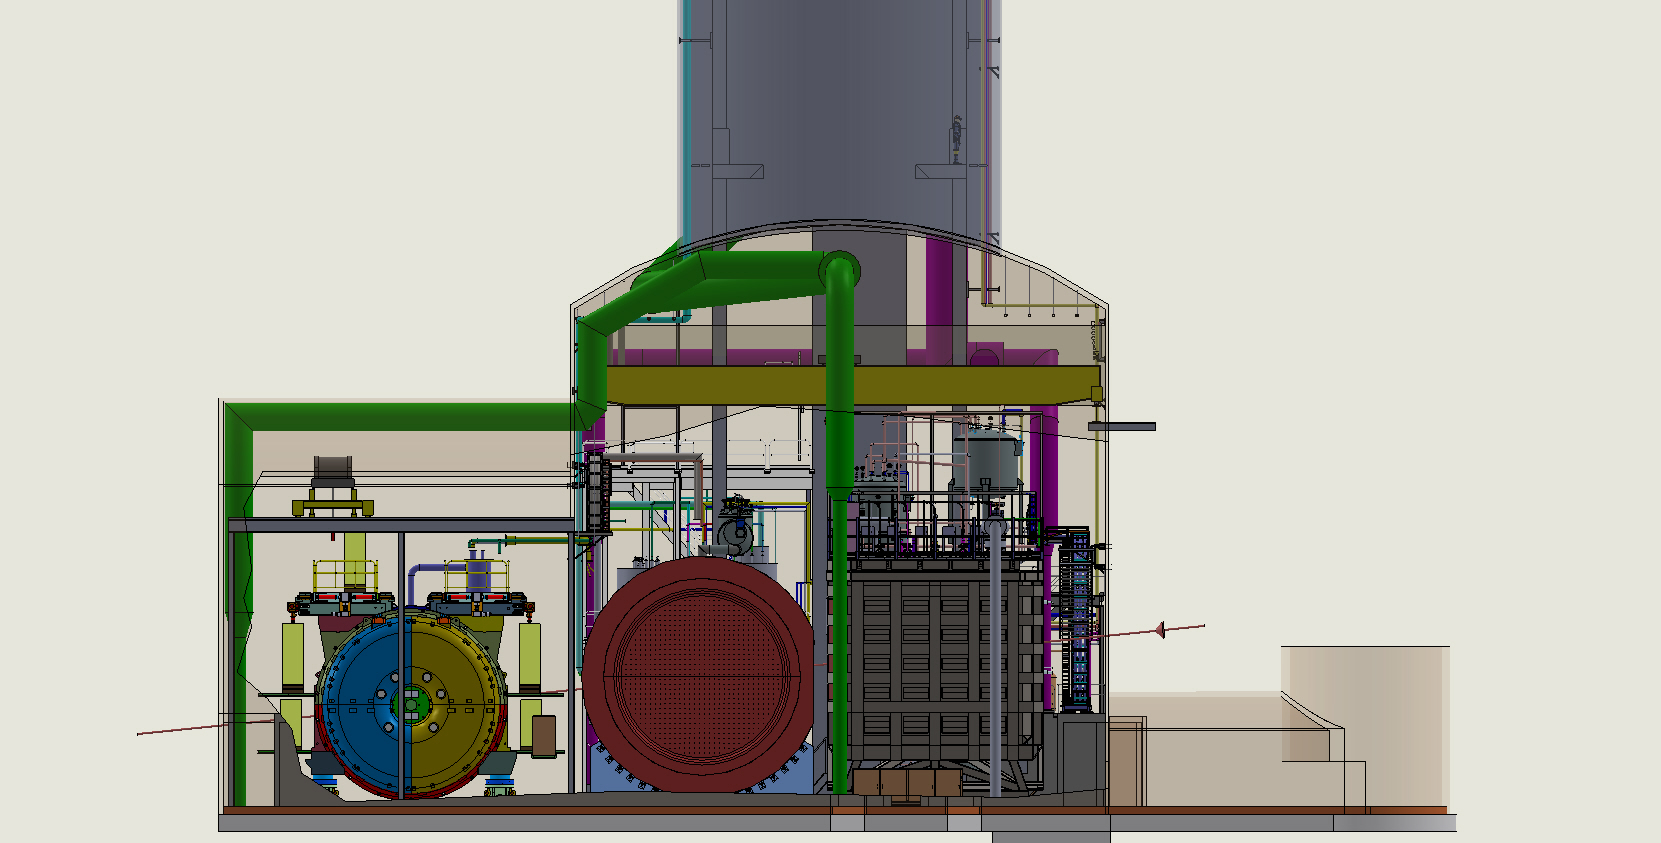
\includegraphics[width=0.9\textwidth]{figures/ch3-DUNE/ndhall.JPG}
     \caption{Schematic representation of the Far Detector experiment with its main components}
        \label{fig:NDhall}
\end{figure}

To enable oscillation measurements, DUNE must first predict the anticipated signal and background at the Far Detector based on oscillation parameters, followed by a comparison with measured flavour-tagged neutrino spectra. To generate this prediction, one must determine the neutrino flux at production, neutrino interaction cross-sections, and detector response—factors all affected by systematic uncertainties requiring constraint. The Near Detector (ND) is tailored to address each prediction component: it will gauge the un-oscillated neutrino beam flux both on-axis and at varying off-axis angles; refine models of neutrino interactions through cross-section and final state topology measurements; model detector responses relative to neutrino energy. Additionally, the ND is designed for operation within a high event rate environment, ensuring the requisite statistical coverage across the full phase-space. The ND will be of three detectors with complementary designs: ND-LAr, which will use a LArTPC technology similar to the FD modules; ND-GAr, a gaseous Argon TPC detector; and SAND, a magnetized beam monitor. ND-LAr and ND-GAr are movable off-axis and will contribute to the DUNE-PRISM program, while SAND remains fixed on-axis. A schematic depiction of the Near Detector, inclusive of all detectors, is presented in Figure \ref{fig:NDhall}. Due to budgetary reasons the ND-GAr detector will become available only during Phase II of the DUNE experiment. A much simpler detector referred to as the Temporary Muon Spectrometer (TMS) will replace it during Phase I. Both ND-GAr and the TMS will be discussed in a dedicated section along-side an alternative and now abandoned Phase I muon spectrometer design called ND-GAr-Lite. 

\begin{figure}[!t]
     \centering
     \begin{subfigure}[b]{0.59\textwidth}
         \centering
         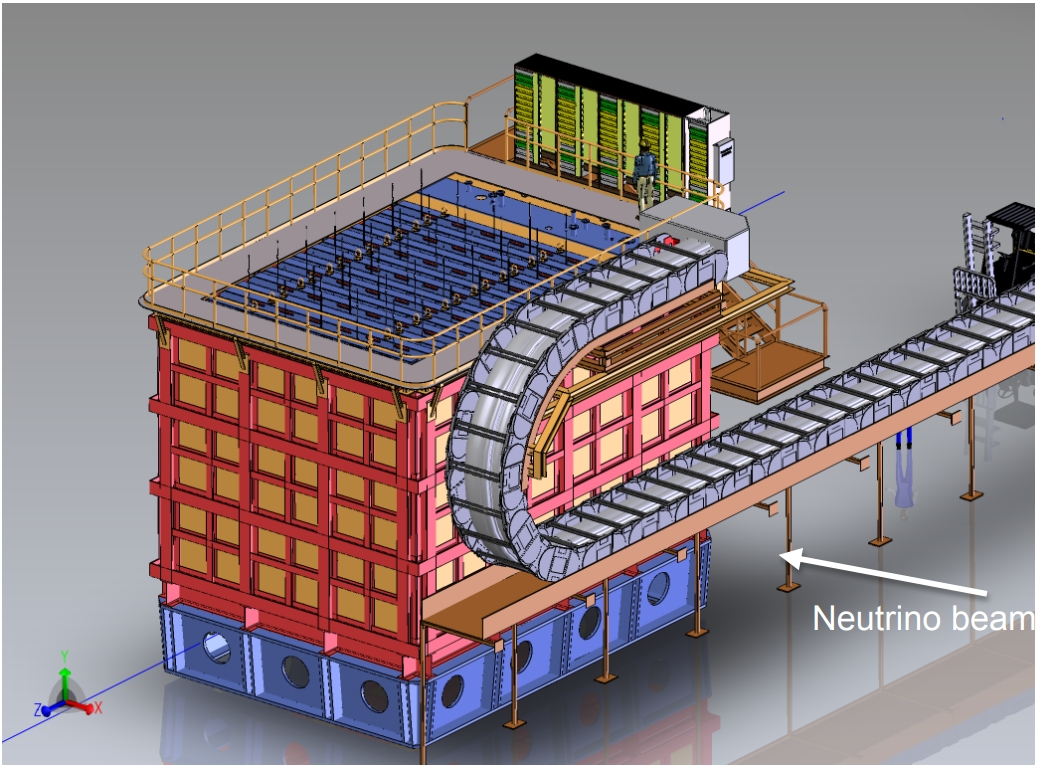
\includegraphics[width=\textwidth]{figures/ch3-DUNE/ND-LAr.jpg}
         \caption{}
         \label{fig:NDLAr}
     \end{subfigure}
     \begin{subfigure}[b]{0.39\textwidth}
         \centering
         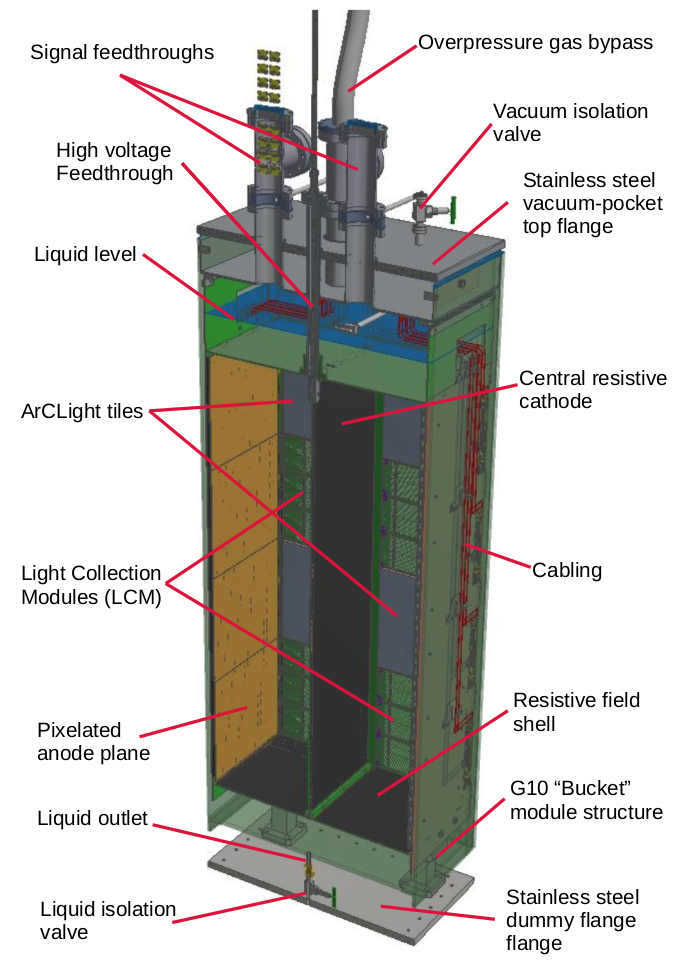
\includegraphics[width=\textwidth]{figures/ch3-DUNE/ND-LAr_module.png}
         \caption{}
         \label{fig:NDLArModule}
     \end{subfigure}
        \caption{(a) Average $\beta$ as a function of the track length $l $ and  (b) average track length as a function of the true momentum $p_\textrm{true}$ for the HP sample.}
        \label{fig:ND-Larview}
\end{figure}

ND-LAr is a LArTPC detector engineered for operation within a high-rate environment. Utilizing the same Argon target and similar detector technology as the FD modules, ND-LAr is essential for modeling detector response and liquid Argon neutrino interaction cross-sections. ND-LAr is comprised of 35 distinct TPC modules, mirroring the design of the ArgonCube prototype \cite{Dwyer:2018phu}. Despite the relativly modest dimentions of the detector, this modular architecture is indispensable for managing the high event rate, facilitating a smaller drift region, enhanced light separation, and increased sensor pixelation. Each module encompasses two optically isolated TPCs outfitted with a LArPix-based pixelated charge readout system  \cite{Goldi:2018mbo}, alongside a light readout for rapid timing data from prompt scintillation light, and a field structure ensuring minimal field non-uniformity throughout the active volume. Given the relatively compact dimensions of its active volume, ND-LAr cannot fully contain the majority of muons generated in $\nu_\mu$ Charged Current (CC) interactions within liquid Argon. Hence, precise momentum reconstruction of this muon sample necessitates an external spectrometer component, a role fulfilled by ND-GAr and the TMS.

\begin{figure}[t]
     \centering
     \begin{subfigure}[b]{0.5\textwidth}
         \centering
         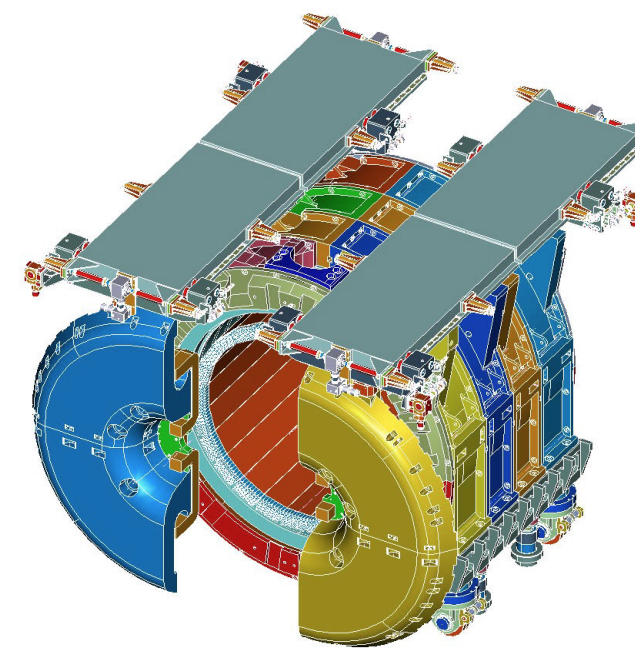
\includegraphics[width=\textwidth]{figures/ch3-DUNE/SAND.png}
         \caption{}
         \label{fig:SAND-outside}
     \end{subfigure}
     \hfill
     \begin{subfigure}[b]{0.48\textwidth}
         \centering
         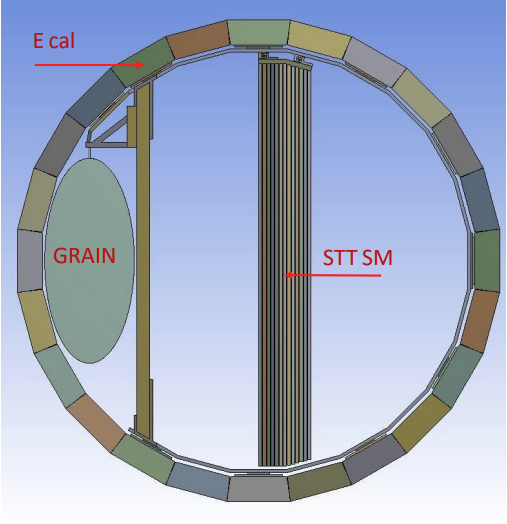
\includegraphics[width=\textwidth]{figures/ch3-DUNE/SAND-inside.png}
         \caption{}
         \label{fig:SAND-inside}
     \end{subfigure}
        \caption{(a) Schematic view of the external components of SAND, including its cryostat and its solenoid magnet (b) Side view of the internal components of SAND, including its active liquid Argon target called GRAIN, one of the straw tube tracker modules and the electro-magnetic calorimeter.  }
        \label{fig:SAND-all}
\end{figure}

ND-LAr and ND-GAr possess the capability to be translated up to 30 meters perpendicular to the neutrino beam axis, spanning angles from $0^{\circ}$ to $3^{\circ}$, a feature named DUNE-PRISM. With increasing off-axis angles, the mean energy of the neutrino flux diminishes while its energy dispersion narrows. Consequently, the Near Detector gains access to diverse un-oscillated neutrino flux profiles, combining them to predict the oscillated flux at the far detector. This data-centric methodology mitigates reliance on models. Moreover, a  of the DUNE-PRISM program is that the off-axis fluxes will variate in mean energies and spreads and will thus be dominated by distinct interaction types (e.g., quasi-elastic, resonant etc.). Access to this variety of samples will facilitate the disentanglement of cross-section effects, enhancing flux and interaction modeling.


The System for On-Axis Neutrino Detection (SAND) will function as a constant on-axis monitor of the neutrino beam, a crucial role for the DUNE-PRISM program. It will ensure that any differences in flux measured by ND-LAr and ND-GAr result from their off-axis position rather than anomalies in beam production. SAND's main structural components, along with its solenoid magnet, cryostat, and electromagnetic calorimeter, will be repurposed from the KLOE experiment (Figure \ref{fig:SAND-all}). The internal tracker design of SAND has recently been finalized, featuring a Straw Tube Tracker (STT) divided in modules. These modules will include a series of tunable passive slabs interleaved with tracking layers of 5mm diameter tubes. SAND will provide various targets, such as CH$_2$ and C, potentially highly useful in studying neutrino interactions. They will offer a clean sample of neutrino-on-hydrogen interactions by "subtraction," devoid of nuclear effects. Additionally, SAND will incorporate its own active target of liquid Argon called GRAIN, whose design is currently being finalized. 

\section{The ND-GAr detector}
\clearpage
\subsection{The ALICE-inspired TPC}
\subsection{The magnet and the high pressure system}
\subsection{The electro-magnetic calorimeter}
\section{The temporary muon spectrometer}
\subsection{ND-GAr-Lite}
\subsection{TMS}
\section{Dune's scientific program}
\subsection{Sensitivities and systematics}
\subsection{Mass ordering and $\delta_\textrm{CP}$}
\subsection{Precision measurements}
\subsection{Proton decay}
\subsection{Supernova neutrinos}
\subsection{Oscillation physics with atmospheric neutrinos}
\subsection{Near Detector Physics}
\subsection{ND-GAr Physics}